
\chapter{Background}

\section{Memory Errors}
Languages like \texttt{C} and \texttt{C++} lack type safety and memory safety which leads to memory corruption errors like stack-based buffer overflow \citep{cwe121}, heap-based buffer overflow \citep{cwe122}, double free \citep{cwe415}, use after free \citep{cwe416}, etc. Memory errors are nothing but the malicious attacks incurred by utilizing the process memory to change the program behavior. Using memory errors, an attacker can change the flow of code and direct it to the attacker specified location, such as shell code, either directly or using gadgets (small instruction chucks) present in the memory to craft malicious attacks. There are a number of solutions proposed to mitigate these vulnerabilities and to ensure memory safety, but none of them are perfect. For example, a well known technique like address space randomization (ASLR) \citep{aslr} can also be exploited, as shown by Strackx et al. \citep{strackx2009breaking}, Shacham et al. \citep{Shacham:2004:EAR:1030083.1030124} and others. \citep{6547101} explains different types of memory errors and effectiveness of their defense mechanisms in details. The program is considered memory safe, if not a single memory related attack is possible. Michael Hicks \citep{memsafetydef} explains the formal definition of memory safety.

Memory errors can be categorized into two types. One being spatial memory errors and other being temporal memory errors \citep{6547101}. By using these two kinds of errors, the attackers can formulate the initial steps for an attack. For example, attackers can overflow the buffer (spatial errors) or they can use the uninitialized memory by dereferencing invalid pointers (temporal errors). Using these methods they can read or write memory locations to perform malicious activities (for e.g. one can overwrite the saved \texttt{eip} to change the control flow of code to a malicious location). Hence, spatial and temporal memory safety is required to stop these violations \citep{memsafetymatpayer}. Consider an example of spatial memory safety violation in \cref{fig:fig21}. A character pointer \texttt{p} has been assigned a memory of 10 bytes. Hence, every valid memory access must be within the bounds of that pointer's assigned memory object, which is 10 bytes from the address of pointer \texttt{p}. As the pointer points out of the bounds of the allocated object, there is clearly an invalid access (both read and write) and therefore a spatial safety violation exists in this case. An example of temporal memory safety violation is shown in \cref{fig:fig22}. The pointer \texttt{p} has been assigned a memory object of 10 bytes. But, the pointer has been freed (and consequently the memory object has been deallocated) before the access. This is an example of use after free \citep{cwe416} vulnerability. Now, the memory object is no longer associated with the pointer and dereferencing such invalid memory is a memory violation. Both spatial and temporal memory safety is important to ensure the program safety. Our implementation currently deals with only spatial memory safety violations and is based on the SoftBound technique \citep{nagarakatte2009softbound}. The following section describes the SoftBound technique in detail.

\begin{figure}
\begin{centering}
\begin{lstlisting}
char *p = malloc(10);
for (int i = 0; i < 15; ++i)
{
  *(p + i) = i + 65;
  printf("%c\n", p[i]);
}
\end{lstlisting}
\caption{Spatial Memory Safety Violation\label{fig:fig21}}
\par\end{centering}
\end{figure}

\begin{figure}
\begin{centering}
\begin{lstlisting}
char *p = malloc(10);
free(p);
for (int i = 0; i < 10; ++i)
{
  *(p + i) = i + 65;
  printf("%c\n", p[i]);
}
\end{lstlisting}
\caption{Temporal Memory Safety Violation\label{fig:fig22}}
\par\end{centering}
\end{figure}

\section{The SoftBound Technique}
The SoftBound \citep{nagarakatte2009softbound} technique is a software based defense mechanism against spatial memory errors. It is a compiler based technique and no source code changes or hardware support is necessary for its implementation. It uses pointer based approach, storing base and bound metadata associated with pointers in a disjoint metadata structure. For e.g., for dynamic memory allocations like \texttt{p = malloc(10)}, the base is assigned to the value of heap pointer returned by Malloc function, i.e. \texttt{p} and bound is assigned to \texttt{p+10}. On every pointer load and store, checks get added to inspect whether the pointer accesses are within the bounds. For e.g.:
\begin{lstlisting}
// Check if the pointer if within the bounds
if ((pointer < pointer_base) || (pointer+size > pointer_bound))
  abort();
// pointer load
a = *pointer;
\end{lstlisting}
Here, the size is the size of the \texttt{pointer} on stack. Check has been added before \texttt{pointer} load to verify whether the \texttt{pointer} access is withing the bounds. Hence, in this way spatial memory protection can be provided. Other features of this technique are metadata propagation, disjoint metadata structure, pointer bounds narrowing, etc. Although our implementation is based on the SoftBound technique, we don't apply compiler transformation techniques (used in SoftBound), as our implementation deals with securing ELF binaries. Therefore, we have to rely on static analysis and dynamic instrumentation frameworks.

\section{Static Binary Analysis and Dynamic Binary Instrumentation Frameworks}

Static and dynamic checks can be added at source code level (i.e. by transforming the source code in to a secure format), during compilation, after linking or during execution (dynamic instrumentation) \citep{luk2005pin}. We assume that we only get the executable as an input (and not the source code). Hence, in our case, it can either be done statically by analyzing binary or dynamically during the run time. There are numerous analysis and instrumentation techniques that are being used to inspect code, add new code, modify existing program or change the control flow, analyse the performance of the program, etc. The following sub-sections explain about well known static binary analysis and dynamic instrumentation frameworks.

\subsection{Dynamic Binary Instrumentation Framework}

Dynamic instrumentation techniques are used to add instrumentation at run time. They use profiling information (dynamic) to analyze binary, which is not available (and possible) in case of static analysis tools (for e.g. variables depend on user input). They can be used for taint analysis, double free detection, control flow modification, data and instruction modification, memory leak detection, etc. \citep{dynamicinstrumentationusage}, using instrumentation and analysis. PIN \citep{luk2005pin}, DynamoRio \citep{bruening2003infrastructure}, Valgrind \citep{nethercote2007valgrind} and Frida \citep{fridaframework} are some of the prominent dynamic instrumentation techniques/ frameworks available today in the market. We use PIN framework to detect spatial errors using dynamic instrumentation techniques.

\subsubsection{PIN Framework}
PIN \citep{luk2005pin} is an instrumentation platform, which can be used to analyze the binary dynamically. It uses JIT (Just In Time) based compilation techniques to instrument binaries at run time. Its implementation is based on the ATOM model \citep{srivastava1994atom}, where the instrumentation routine is used to determine the places in the code to be analyzed and the analysis routine actually analyzes the procedural information. Pin tool is written in \texttt{C++} (about 99\%) and \texttt{assembly} (about 1\%) and is compatible across multiple architectures (Though, the source code is private). PIN has an architecture independent API, but the architecture specific details can be accessed with ease. Using this API, "instrumentation tools" or "PIN tools" can be built in \texttt{C/C++} to add instrumentation, to modify and analyze binaries. Another advantage of PIN is that, it can be attached to (and detached from) the running process as well (using "Ptrace" technique). PIN can be used to analyze the binary, simply by the following command:

\begin{lstlisting}
pin -t yourtool.so -- yourbinary
\end{lstlisting}
Here, "pin" is the PIN framework (an executable), "yourtool.so" is the PIN tool and "yourbinary" is the binary to be analyzed. Hence, as the user runs PIN, three binaries run together - PIN framework, Pintool (instrumentation tool written by the user) and the binary to be analyzed. They also share the same address space (but they have their own copies of libraries, i.e. the libraries are not shared). Every time PIN is run, the PIN framework translates the input code using dynamic (JIT) compilation. The code which gets executed is always the translated code and not the original code. The instrumentation is added by Pintool during the translation, and hence the translated code contains instrumentation (only if it has been added previously). The instrumentation and analysis routines are defined in the Pintool. Translated code is stored in the code cache, which can be used to run the frequently executed code, without any need of re-translation. Code cache improves the overall performance.

An example Pintool (based on a similar example given in the PIN user guide \citep{intelpinuserguide}) is shown in \cref{fig:fig23}. It counts the total number of instructions executed by instrumenting at the instruction level granularity. As seen in the example code, the function \texttt{Instruction} is equivalent to the instrumentation routine and the function \texttt{docount} is equivalent to the analysis routine, according to the ATOM model.

\begin{figure}
\begin{centering}
\begin{lstlisting}
#include "pin.H"

// Instructions count is kept here
static UINT64 icount = 0;

// docount is called before every instruction gets executed
// This is equivalent to the analysis routine in the ATOM model
VOID docount()
{
  icount++;
}

// Call for every new instruction
// This is equivalent to the instrumentation routine in the ATOM model
// This can be used to decide when to add an analysis routine
VOID Instruction(INS ins, VOID *v)
{
    // Insert a call to docount before every instruction
    INS_InsertCall(ins, IPOINT_BEFORE, (AFUNPTR)docount, IARG_END);
}

int main(int argc, char * argv[])
{
    // Initialize pin
    PIN_Init(argc, argv);
    // This function adds instrumentation for every detected instruction
    INS_AddInstrumentFunction(Instruction, 0);
    PIN_StartProgram();
    return 0;
}
\end{lstlisting}
\caption{A Simple Pintool To Count Total Number Of Executed Instructions\label{fig:fig23}}
\par\end{centering}
\end{figure}

\subsection{Static Binary Analysis and Reverse Engineering Tools}
Static binary analysis is analyzing binaries without executing them. Frameworks like Ghidra \citep{nsaghidra}, Radare2 \citep{radare2}, Binary Ninja \citep{binaryninja}, Hopper \citep{hopper}, IDA pro \citep{idapro}, etc. use reverse engineering techniques to explore binary information. Some of them are open source, while others are closed source. They make use of symbol information in present in an executable to make their analysis better. In our implementation, we use Ghidra, along with PIN.

\subsubsection{Ghidra Framework}
Ghidra is NSA's (National Security Agency) reverse engineering framework, released recently on April 4, 2019. It is primarily written in Java and supports multiple operating systems such as Windows, Linux and MacOS. It can be run in GUI (graphical user interface) as well as command-line mode. An example window of Ghidra in GUI mode (using eclipse) is shown in \cref{fig:fig24}. Ghidra comes with a number of tools, which offer disassembly, decompilation, scripting, code modifications, data type management and plenty of other analysis. Scripting is currently supported in Java and Python languages with the availability of a rich API. Custom scripts can be run pre-analysis or post-analysis. Ghidra also supports multi-user environment which is a good option for users who would like to work in team on a same project.

\begin{figure}
\centering
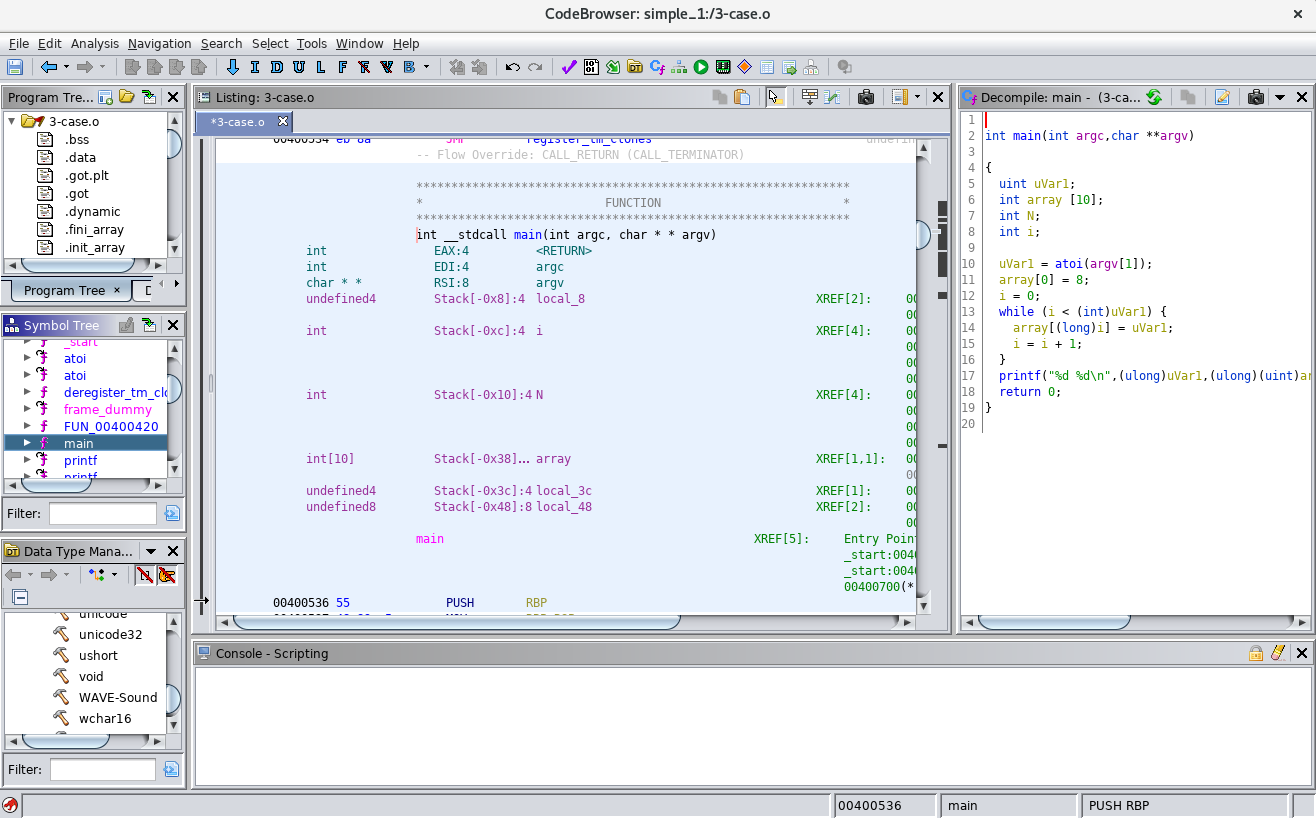
\includegraphics[width=165mm]{images/ghidra.png}
\caption{Ghidra - Graphical User Interface\label{fig:fig24}}
\end{figure}